\documentclass[11pt,letterpaper]{article}

\usepackage[margin=0.8in]{geometry}
\usepackage[T1]{fontenc}
\usepackage{lmodern}
\usepackage{microtype}
\usepackage{graphicx}
\usepackage{booktabs}
\usepackage{tabularx}
\usepackage{array}
\usepackage{float}
\usepackage{enumitem}
\usepackage{xcolor}
\usepackage{hyperref}
\usepackage{caption}
\usepackage{listings}
\hypersetup{colorlinks=true,linkcolor=blue!45!black,citecolor=blue!45!black,urlcolor=blue!45!black}
\graphicspath{{images/}}
\setlength{\parskip}{0.45em}
\setlength{\parindent}{0pt}
\captionsetup{font=small,labelfont=bf}
\renewcommand{\arraystretch}{1.2}
\newcolumntype{Y}{>{\raggedright\arraybackslash}X}
\newcommand{\memberA}{[Member 1 name, student ID]}
\newcommand{\memberB}{[Member 2 name, student ID]}
\newcommand{\memberC}{[Member 3 name, student ID]}
\newcommand{\project}{InfoVis Explorer}

\title{\textbf{Interactive Information Visualization of Clickstream and Housing-Market Data}\\[0.4em]
\large DAS732 Data Visualization -- Assignment 2, Task 2}
\author{\memberA \and \memberB \and \memberC}
\date{Term 1, 2026--27}

\begin{document}
\maketitle
\begin{abstract}
This report documents the design, implementation, and interpretation of the InfoVis component of Assignment 2. The work uses two complementary datasets: directed Wikipedia clickstream transitions to study a network, and Redfin metro-level monthly housing indicators to study multivariate, hierarchical, and temporal patterns. The browser application combines a NetworkX-generated node-link analysis with three graph layouts and interactive filtering; JavaScript parallel coordinates with edge bundling and brushing; zoomable treemaps under two alternative hierarchies; and Python-generated horizon and ridgeline plots, with two variations of each. We describe data preparation and sampling explicitly, connect findings to the figures, discuss interaction and visual encoding choices, and identify limitations that affect interpretation. The source is intended to be compiled from the \texttt{task2} directory; names and contributions below are editable placeholders.
\end{abstract}

\tableofcontents
\newpage

\section{Introduction and objectives}
InfoVis Task 2 asks for a network visualization with at least three compared layouts and interaction, browser-based JavaScript visualizations for parallel coordinates with edge bundling and zoomable treemaps, and Python-library visualizations of horizon and ridgeline plots. Each method should be supported by appropriate data, complete visual labeling, and written inferences. The assignment also emphasizes preprocessing, high-resolution figure files, and individual team contributions \cite{assignment}.

The project, \project, uses a large clickstream as a directed network and the Redfin housing data supplied with the A1 work for the other views. These sources answer different questions. Clickstream edges represent observed transitions between pages, while Redfin records describe monthly market conditions for metropolitan areas. The dashboard is organized into four views: Network, Parallel coordinates, Zoomable treemaps, and Horizon and ridgeline. The report's aims are to (1) explain how the data were transformed, (2) document the encoding and interaction choices, (3) compare the required visual alternatives, and (4) make evidence-based observations without treating association as causation.

\subsection{Questions explored}
\begin{enumerate}[leftmargin=*]
  \item Which high-activity clickstream pages and transitions form a useful core network, and how does the choice of layout affect its readability?
  \item How do Redfin metro markets differ across price, activity, inventory, and selling-time measures, and how can brushing and bundling help inspect those relationships?
  \item How do market size and geographic hierarchy affect the interpretation of housing-market totals and indicators in a treemap?
  \item How did metro-level prices and time on market vary over 2020--2026, and how do patterns differ by metro size and Census region?
\end{enumerate}

\section{Assignment coverage}
Table~\ref{tab:coverage} maps each InfoVis requirement to the implemented method and report evidence. The visualizations and source code are included in the accompanying project; figures cited below are also available as standalone image files in \texttt{task2/images}.

\begin{table}[H]
\centering\small
\begin{tabularx}{\textwidth}{p{0.26\textwidth}YY}
\toprule
\textbf{Requirement} & \textbf{Implementation} & \textbf{Evidence in this report} \\
\midrule
NetworkX node-link diagram; sufficiently complex network; compare at least three layouts and provide interaction & 120-page directed click-flow core; Spring, Kamada--Kawai, ForceAtlas2; filtering, search, hover, selection and neighbor highlighting & Figure~\ref{fig:layouts}; Section~\ref{sec:network} \\
JavaScript parallel coordinates with edge bundling and user interaction & Redfin multivariate records; median-profile bundling; draggable axes and brushes & Figure~\ref{fig:parallel}; Section~\ref{sec:parallel} \\
JavaScript zoomable treemap and alternative tabular-to-tree remodels & State--metro and market-tier--state--metro hierarchies; selectable area and color measures; zoom and breadcrumbs & Figure~\ref{fig:treemap}; Section~\ref{sec:treemap} \\
Python horizon plots, at least two variations & Monthly price change by fixed metro-size tiers; monthly days-on-market change by Census region & Figures~\ref{fig:horizon-price} and~\ref{fig:horizon-dom}; Section~\ref{sec:temporal} \\
Python ridgeline plots, at least two variations & Annual metro price distributions; recent days-on-market distributions by fixed metro-size tier & Figures~\ref{fig:ridge-price} and~\ref{fig:ridge-dom}; Section~\ref{sec:temporal} \\
Data handling, figures, inferences, codebase, references and individual contributions & Reproducible preparation scripts and processed data; figure-linked discussion; editable contribution table & Sections~\ref{sec:data}--\ref{sec:contrib}; References \\
\bottomrule
\end{tabularx}
\caption{Coverage of the InfoVis requirements in the assignment brief.}
\label{tab:coverage}
\end{table}

\section{Data sources and preparation}\label{sec:data}
\subsection{Wikipedia clickstream network}
The input \texttt{clickstream\_data1.tsv} contains source page, destination page, referrer or relationship type, and click count. Each row is an aggregated transition count rather than an individual user event. The data do not provide a timestamp suitable for a time-series analysis; therefore, time-series views use Redfin instead. This distinction prevents interpreting click counts as unique people or a chronological sequence of visits.

The source contains 32,292,988 records and 7,035,369,921 clicks across all relationship classes. The network view focuses on the internal \texttt{link} class, which has 22,368,108 records and 2,275,646,017 clicks. Pages are ranked by total incoming plus outgoing click activity; the 120 highest-activity pages are retained as nodes. Directed link records between those selected pages are aggregated into weighted edges. The resulting induced core has 558 directed edges and 13,875,822 clicks, approximately 0.61\% of all internal-link clicks. All observed internal-link edges among the selected nodes are retained, including lower-volume edges; the dashboard's edge threshold is an interactive display filter.

This reduction makes an interactive view practical and focuses attention on prominent pages, but it is intentionally activity-biased. It does not represent the full long tail of pages. The node selection uses total in- and out-activity, while displayed link weights come only from internal-link transitions; the selection and edge populations therefore have different scopes. These are important qualifications when interpreting the graph.

\subsection{Redfin metro-month housing data}
The input \texttt{redfin\_housing.csv} contains 75,665 metro-month observations for 946 metro areas across 51 state or District of Columbia codes, covering January 2020 through August 2026 (80 months). It includes market measures such as median sale price, year-over-year (YoY) price change, homes sold, active listings, inventory, pending sales, days on market (DOM), and months of supply. Fifteen metro-month cells are absent. Field-level missingness is modest but nonzero: homes sold and median sale price are each missing in about 0.73\% of rows, DOM in 0.79\%, active listings in 0.11\%, and inventory in 0.14\%.

Metro names are parsed to derive two-letter state codes and Census regions. A stable four-level metro-size tier is based on each metro's median monthly homes sold during 2024--2025, yielding 237 small-volume, 236 medium-low, 236 medium-high, and 237 high-volume metros. Fixed tiers support comparisons across months without redefining group membership as market activity changes. The parallel-coordinates view excludes a metro for a selected month when it lacks a value on any displayed quantitative axis; consequently, its plotted record count can vary with month and selected measures.

For time-series plots, the horizon views aggregate monthly observations using group medians. The annual price ridgeline first obtains an annual median price per metro, then compares the distributions across years. The DOM ridgeline obtains one median DOM per metro over the latest 12 months (September 2025--August 2026) and compares those values by the fixed size tiers. The 2026 annual price distribution is partial because data end in August 2026.

\begin{table}[H]
\centering\small
\begin{tabularx}{\textwidth}{p{0.2\textwidth}p{0.29\textwidth}Y}
\toprule
\textbf{Dataset} & \textbf{Prepared scope} & \textbf{Main transformation and use} \\
\midrule
Clickstream & 32.3M source records; 120 selected pages and 558 induced directed edges in the graph & Aggregate link clicks by directed page pair; derive activity totals and Louvain communities; retain weighted core network. \\
Redfin & 75,665 metro-month rows; 946 metros; Jan 2020--Aug 2026 & Parse geography; derive fixed market-size tiers; calculate group medians, annual metro medians, and rolling-year metro DOM medians for the temporal views. \\
\bottomrule
\end{tabularx}
\caption{Data used and principal preparation steps.}
\label{tab:data}
\end{table}

\section{Methods and implementation}
\subsection{NetworkX node-link diagram}\label{sec:network}
The click-flow network is a directed weighted graph. Node area represents total incoming plus outgoing activity in the selected core. Edge width represents the number of clicks on that directed transition, and node color represents a Louvain community assignment. Arrows preserve direction. Labels are reserved for high-activity or searched pages to reduce visual clutter. The page search locates a node; hovering reports its title, activity, degree, and incident transitions; clicking a node highlights its immediate in- and out-neighbors; and a clear control resets selection.

Three algorithms place the same node and edge set. Spring (Fruchterman--Reingold) models edges as attractive forces and nodes as repelling elements; the layout uses a logarithmic transform of edge weight so the largest click counts do not dominate without bound. Kamada--Kawai optimizes a geometric objective based on shortest-path distances, where high-weight edges are converted to shorter distances. ForceAtlas2 uses a force-directed model and logarithmically scaled click weights. Disconnected nodes are placed around the periphery so that they remain discoverable. The layout selector, visible-page slider (30--120), minimum-click threshold, search, label toggle, hover, and neighbor selection make the comparison interactive.

\begin{figure}[H]
\centering
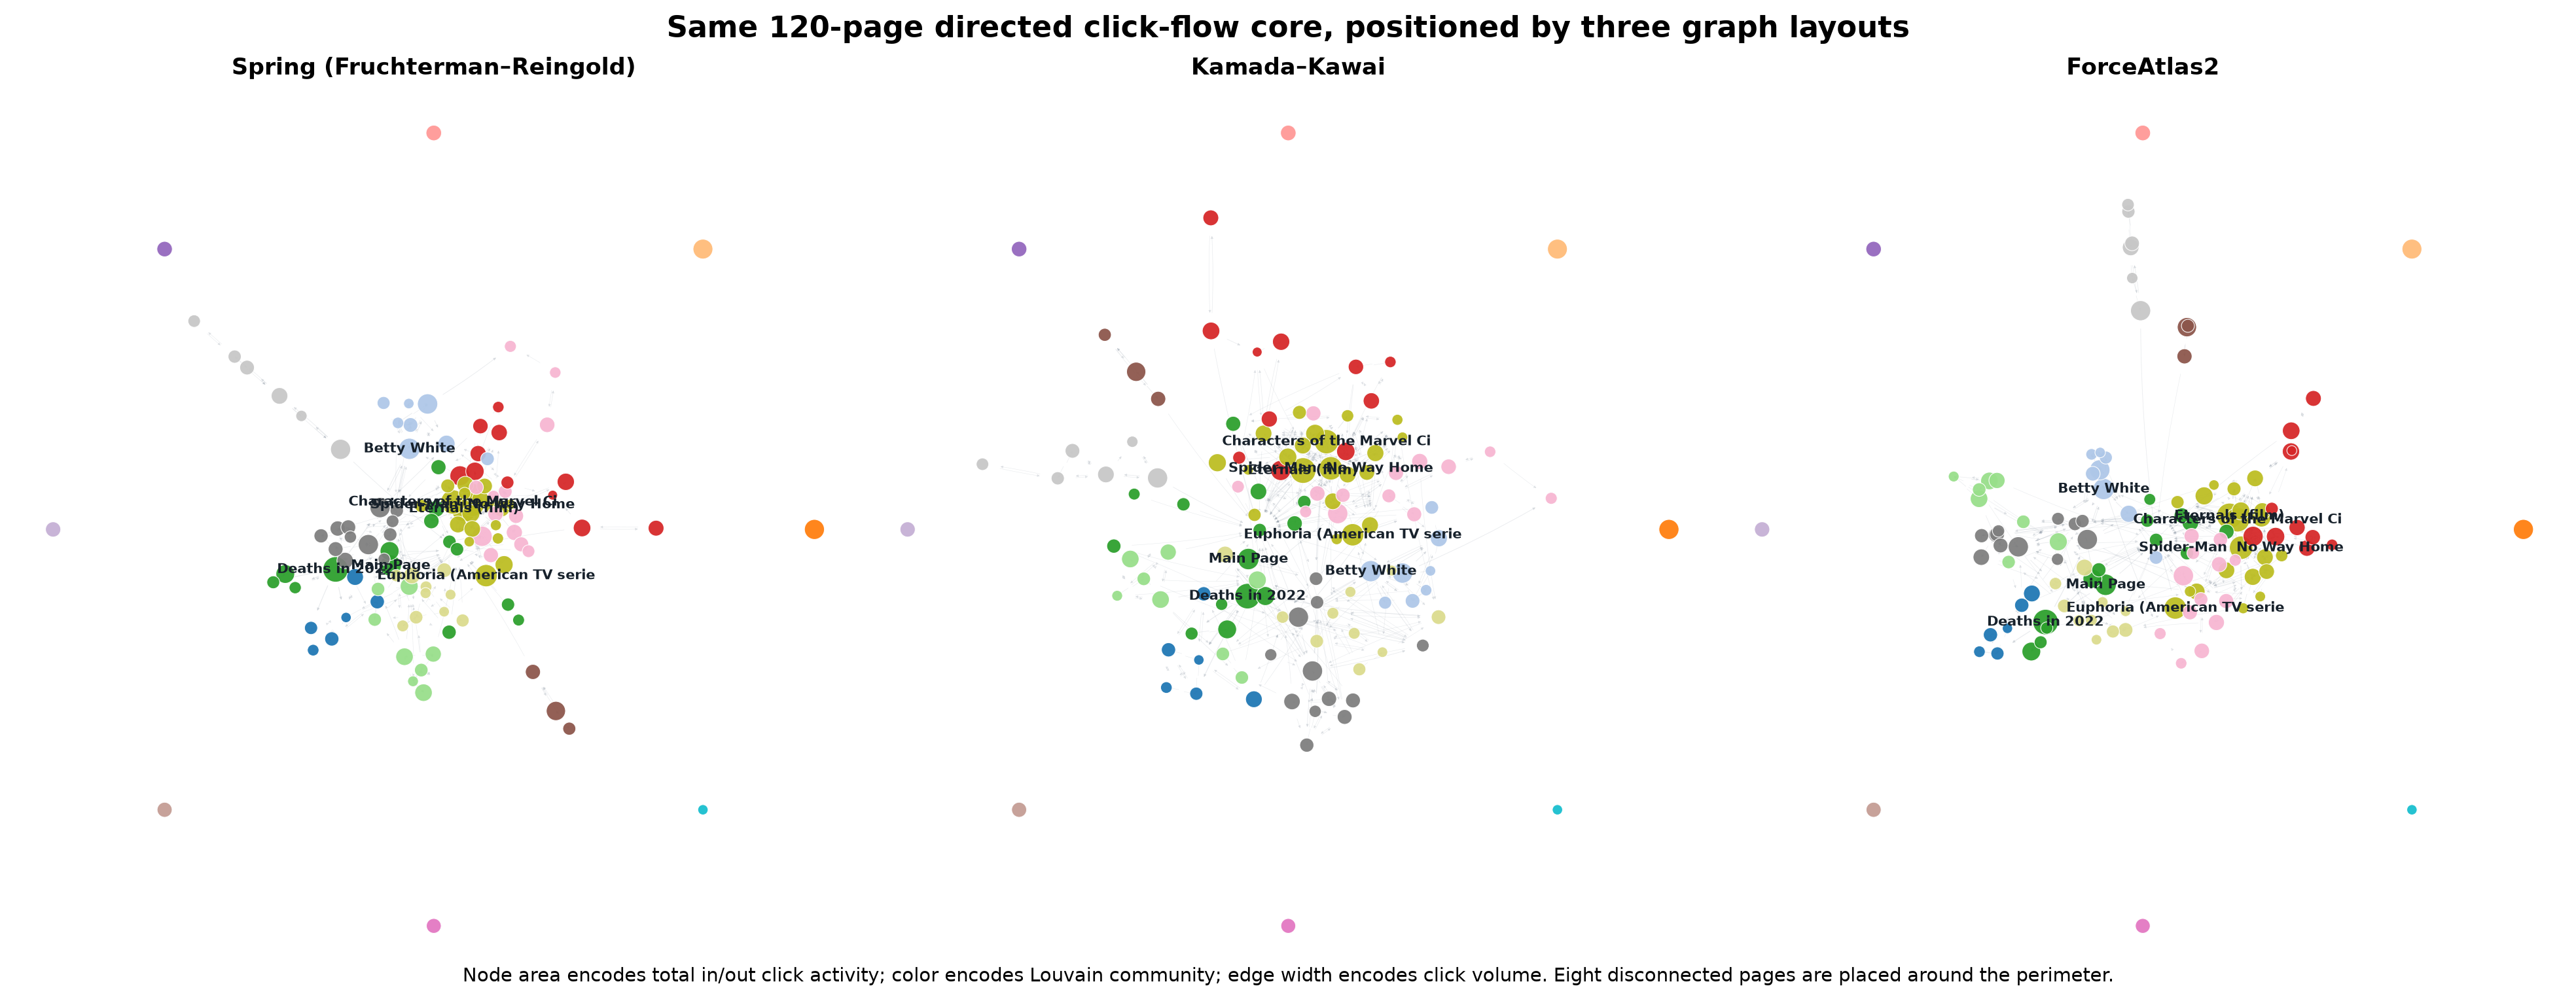
\includegraphics[width=\textwidth]{fig_network_layout_comparison.png}
\caption{The same 120-page directed click-flow core arranged with Spring, Kamada--Kawai, and ForceAtlas2. Node size encodes total in/out activity, color encodes community, and edge width encodes click volume. This static comparison supports layout inspection; the dashboard provides the interactive graph.}
\label{fig:layouts}
\end{figure}

Figure~\ref{fig:layouts} shows that the three methods produce different spatial arrangements while preserving the same underlying relationships. Spring gives a compact force-balanced view; Kamada--Kawai tends to emphasize graph-distance structure; ForceAtlas2 expands the force-directed structure and can expose peripheral nodes. Dense labels and crossings remain difficult in all layouts, which is why search, filtering, and neighbor highlighting are part of the dashboard rather than relying on the static image alone. The layouts do not encode geographic position or a temporal sequence.

The activity ranking identifies \emph{Eternals (film)}, \emph{Deaths in 2022}, and Marvel Cinematic Universe character pages among the most active nodes. The strongest displayed transition is Main Page $\rightarrow$ \emph{Deaths in 2022}; another prominent transition connects \emph{Eternals} to the Marvel character page. Such edges describe aggregated click-flow volume within the chosen core, not a causal relationship between topics or the behavior of a typical individual.

\subsection{Parallel coordinates with edge bundling}\label{sec:parallel}
The parallel-coordinates view is implemented in JavaScript using D3. Each metro is a polyline across axes for median sale price, YoY sale-price change, homes sold, active listings, DOM, months of supply, and fixed market-size tier. Long-tailed positive measures are transformed with $\log_{10}(x+1)$ (price uses a log transform); numeric domains use the 2nd and 98th percentiles to reduce the influence of extreme values, and plotted values are clamped to those display bounds. Tooltips preserve the underlying values.

Edge bundling is implemented by drawing each metro's line through intermediate positions that are pulled toward the median transformed profile for its market-size tier. The amount of pull is controlled by a bundling-strength control; the two endpoints remain attached to the actual axis values. This is a visual simplification that can reveal common profiles, but it can obscure individual outliers, so users can reduce the strength and inspect metros using tooltips. Axis dragging reorders dimensions. A vertical brush on an axis filters records, and brushes can be combined; tier controls further restrict the visible groups. These interactions satisfy the assignment's requirement for user interaction (both axis reordering and brushing are included).

\begin{figure}[H]
\centering
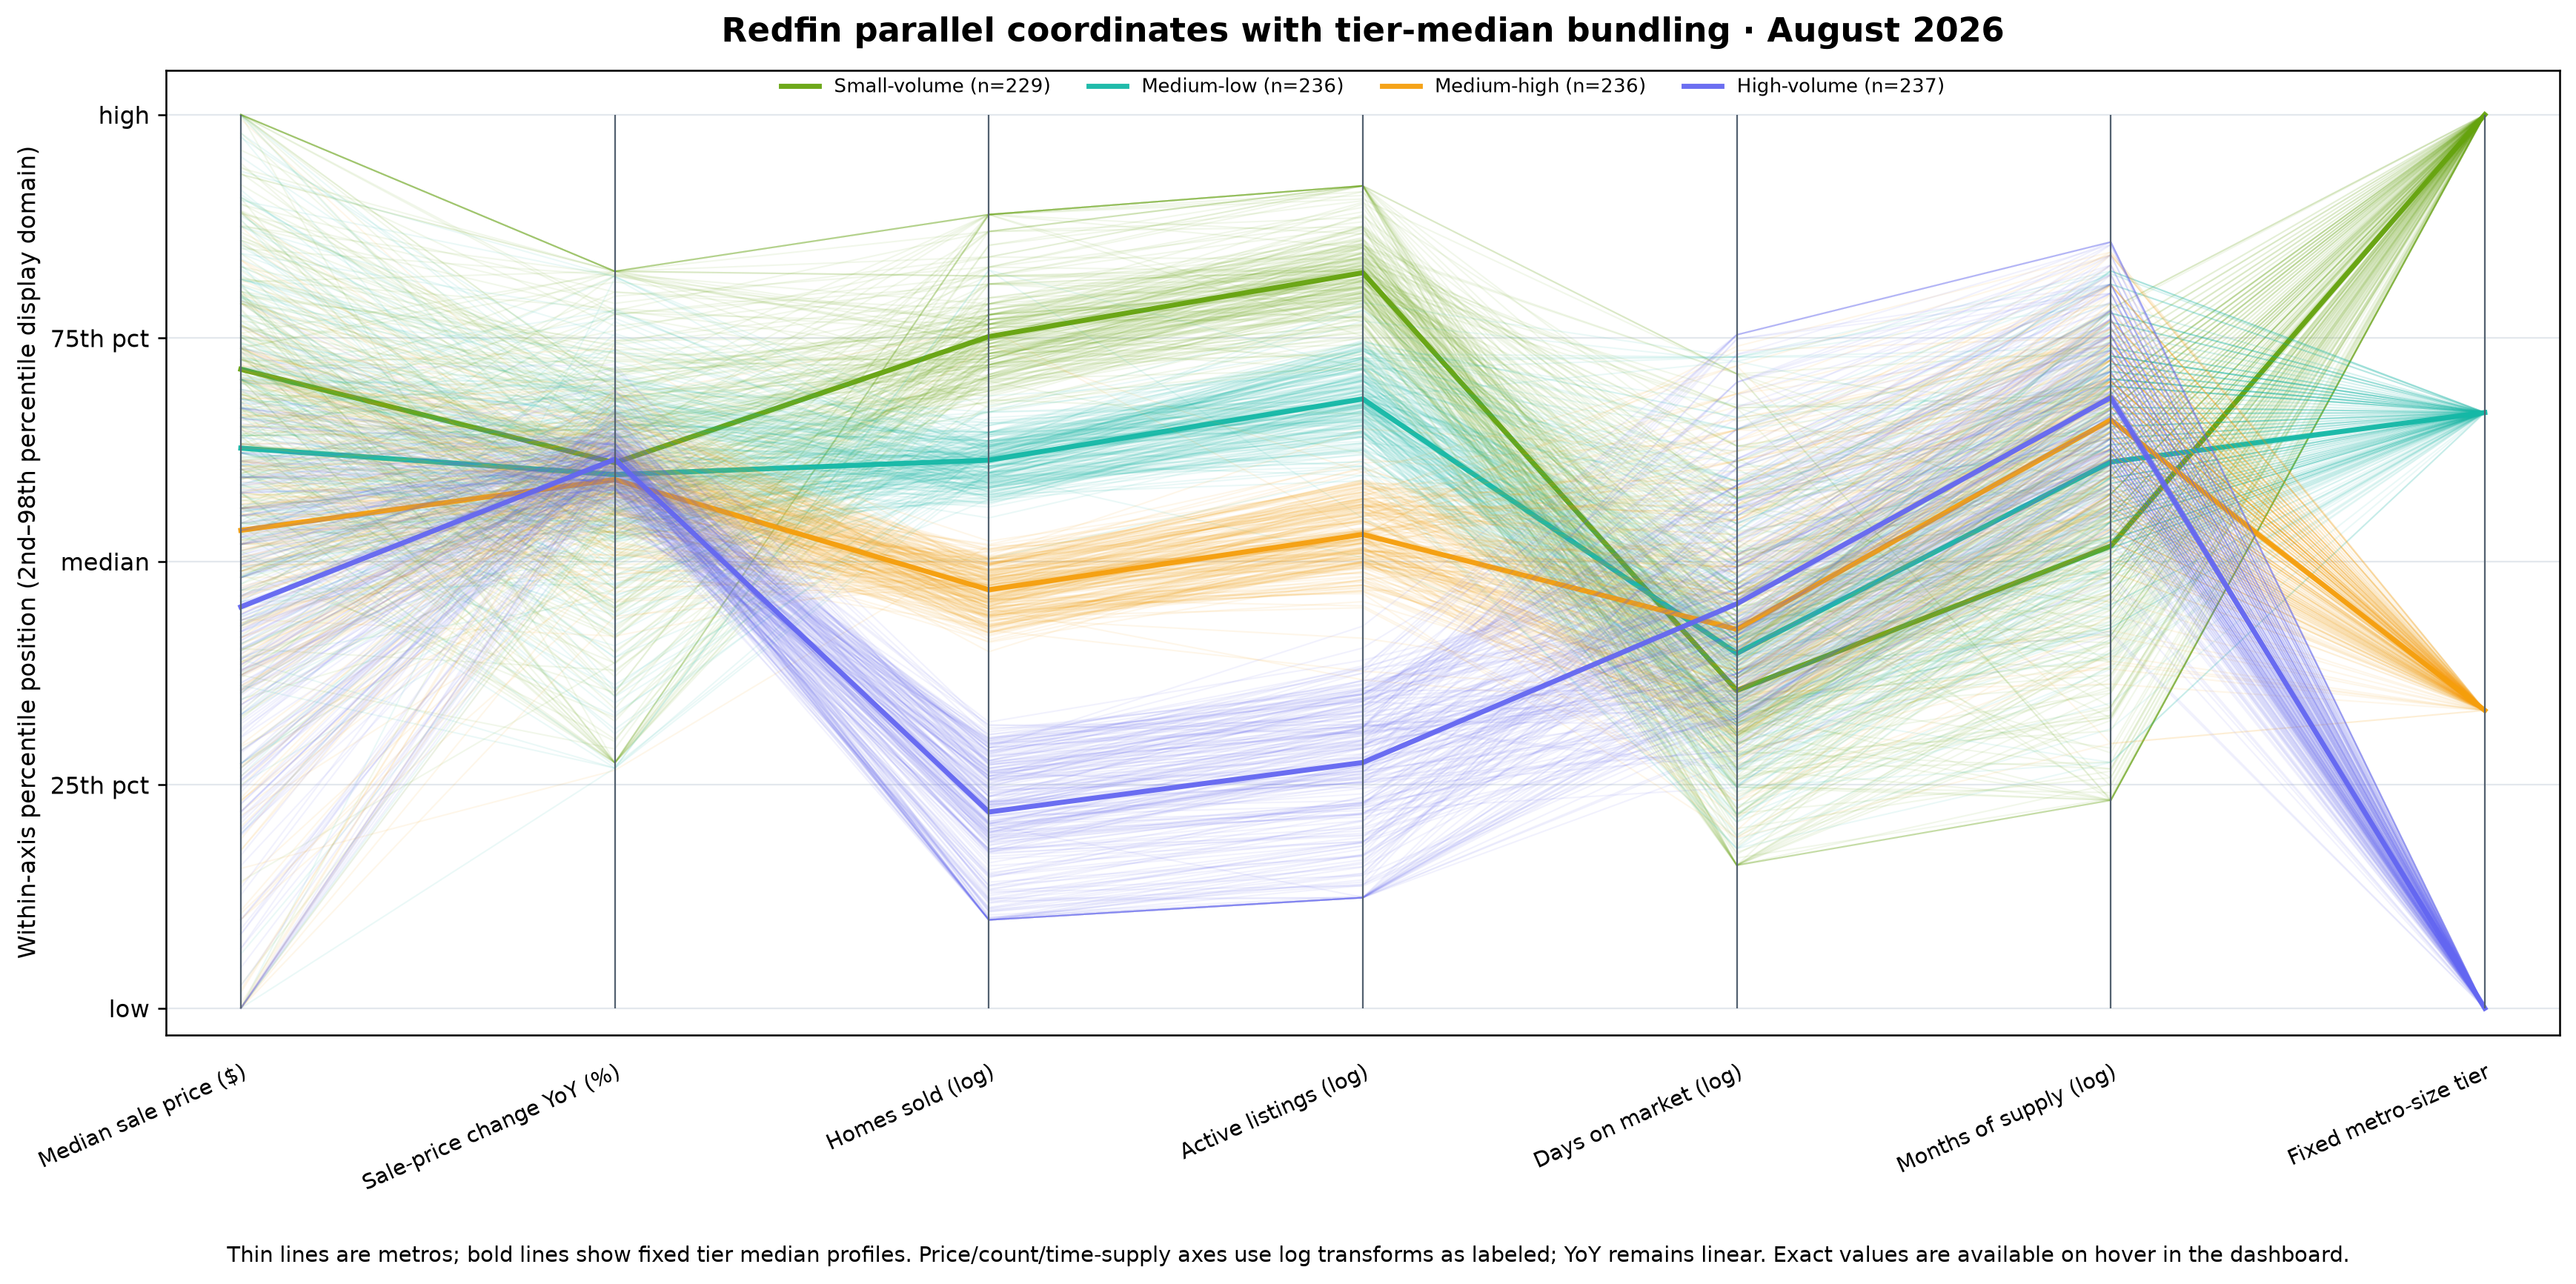
\includegraphics[width=\textwidth]{fig_parallel_coordinates_bundling.png}
\caption{Redfin metro profiles across market indicators. The representative plot uses bundled lines, with tier profiles used as visual anchors; the browser view supports axis reordering, brushing, tier filters, and exact-value tooltips.}
\label{fig:parallel}
\end{figure}

In Figure~\ref{fig:parallel}, the most useful reading is coordinated rather than pointwise: a brush on price, for example, can reveal how the selected metros distribute across sales activity, DOM, inventory, and months of supply. Bundling makes shared tier profiles easier to see than a fully overlapping set of independent lines. Any conclusion from a bundled segment should be checked against the axis endpoints and selected records because intermediate geometry is deliberately adjusted for legibility.

\subsection{Zoomable treemaps}\label{sec:treemap}
The treemap is a browser visualization built with D3 hierarchy and treemap modules. It supports two alternative remodels of the same tabular data: (1) state $\rightarrow$ metro, and (2) market-size tier $\rightarrow$ state $\rightarrow$ metro. The first emphasizes geographic grouping; the second makes market-size groupings explicit while retaining geography. In both, the selected leaf area is an additive monthly measure (homes sold, active listings, inventory, pending sales). The user selects a month and a color measure (median sale price, YoY price change, or DOM). Clicking a parent zooms into it; breadcrumbs navigate back; hovering reports the selected metro or group and its metrics.

For parent groups, area is the sum of the selected additive measure. Color is an area-weighted mean of the metro-level indicator, which provides a coherent summary of the displayed leaves but is not necessarily an official state-level statistic. For example, a parent color labeled by median sale price is a weighted mean of metro medians, not the median of all home sales in that state. To keep tiles readable, color uses a sequential scheme for positive measures and a single-hue red sequential scheme for signed YoY change, with the central 5th--95th percentile range clamped for color. Hover details retain exact values and prevent the clipped color domain from being mistaken for the data range.

\begin{figure}[H]
\centering
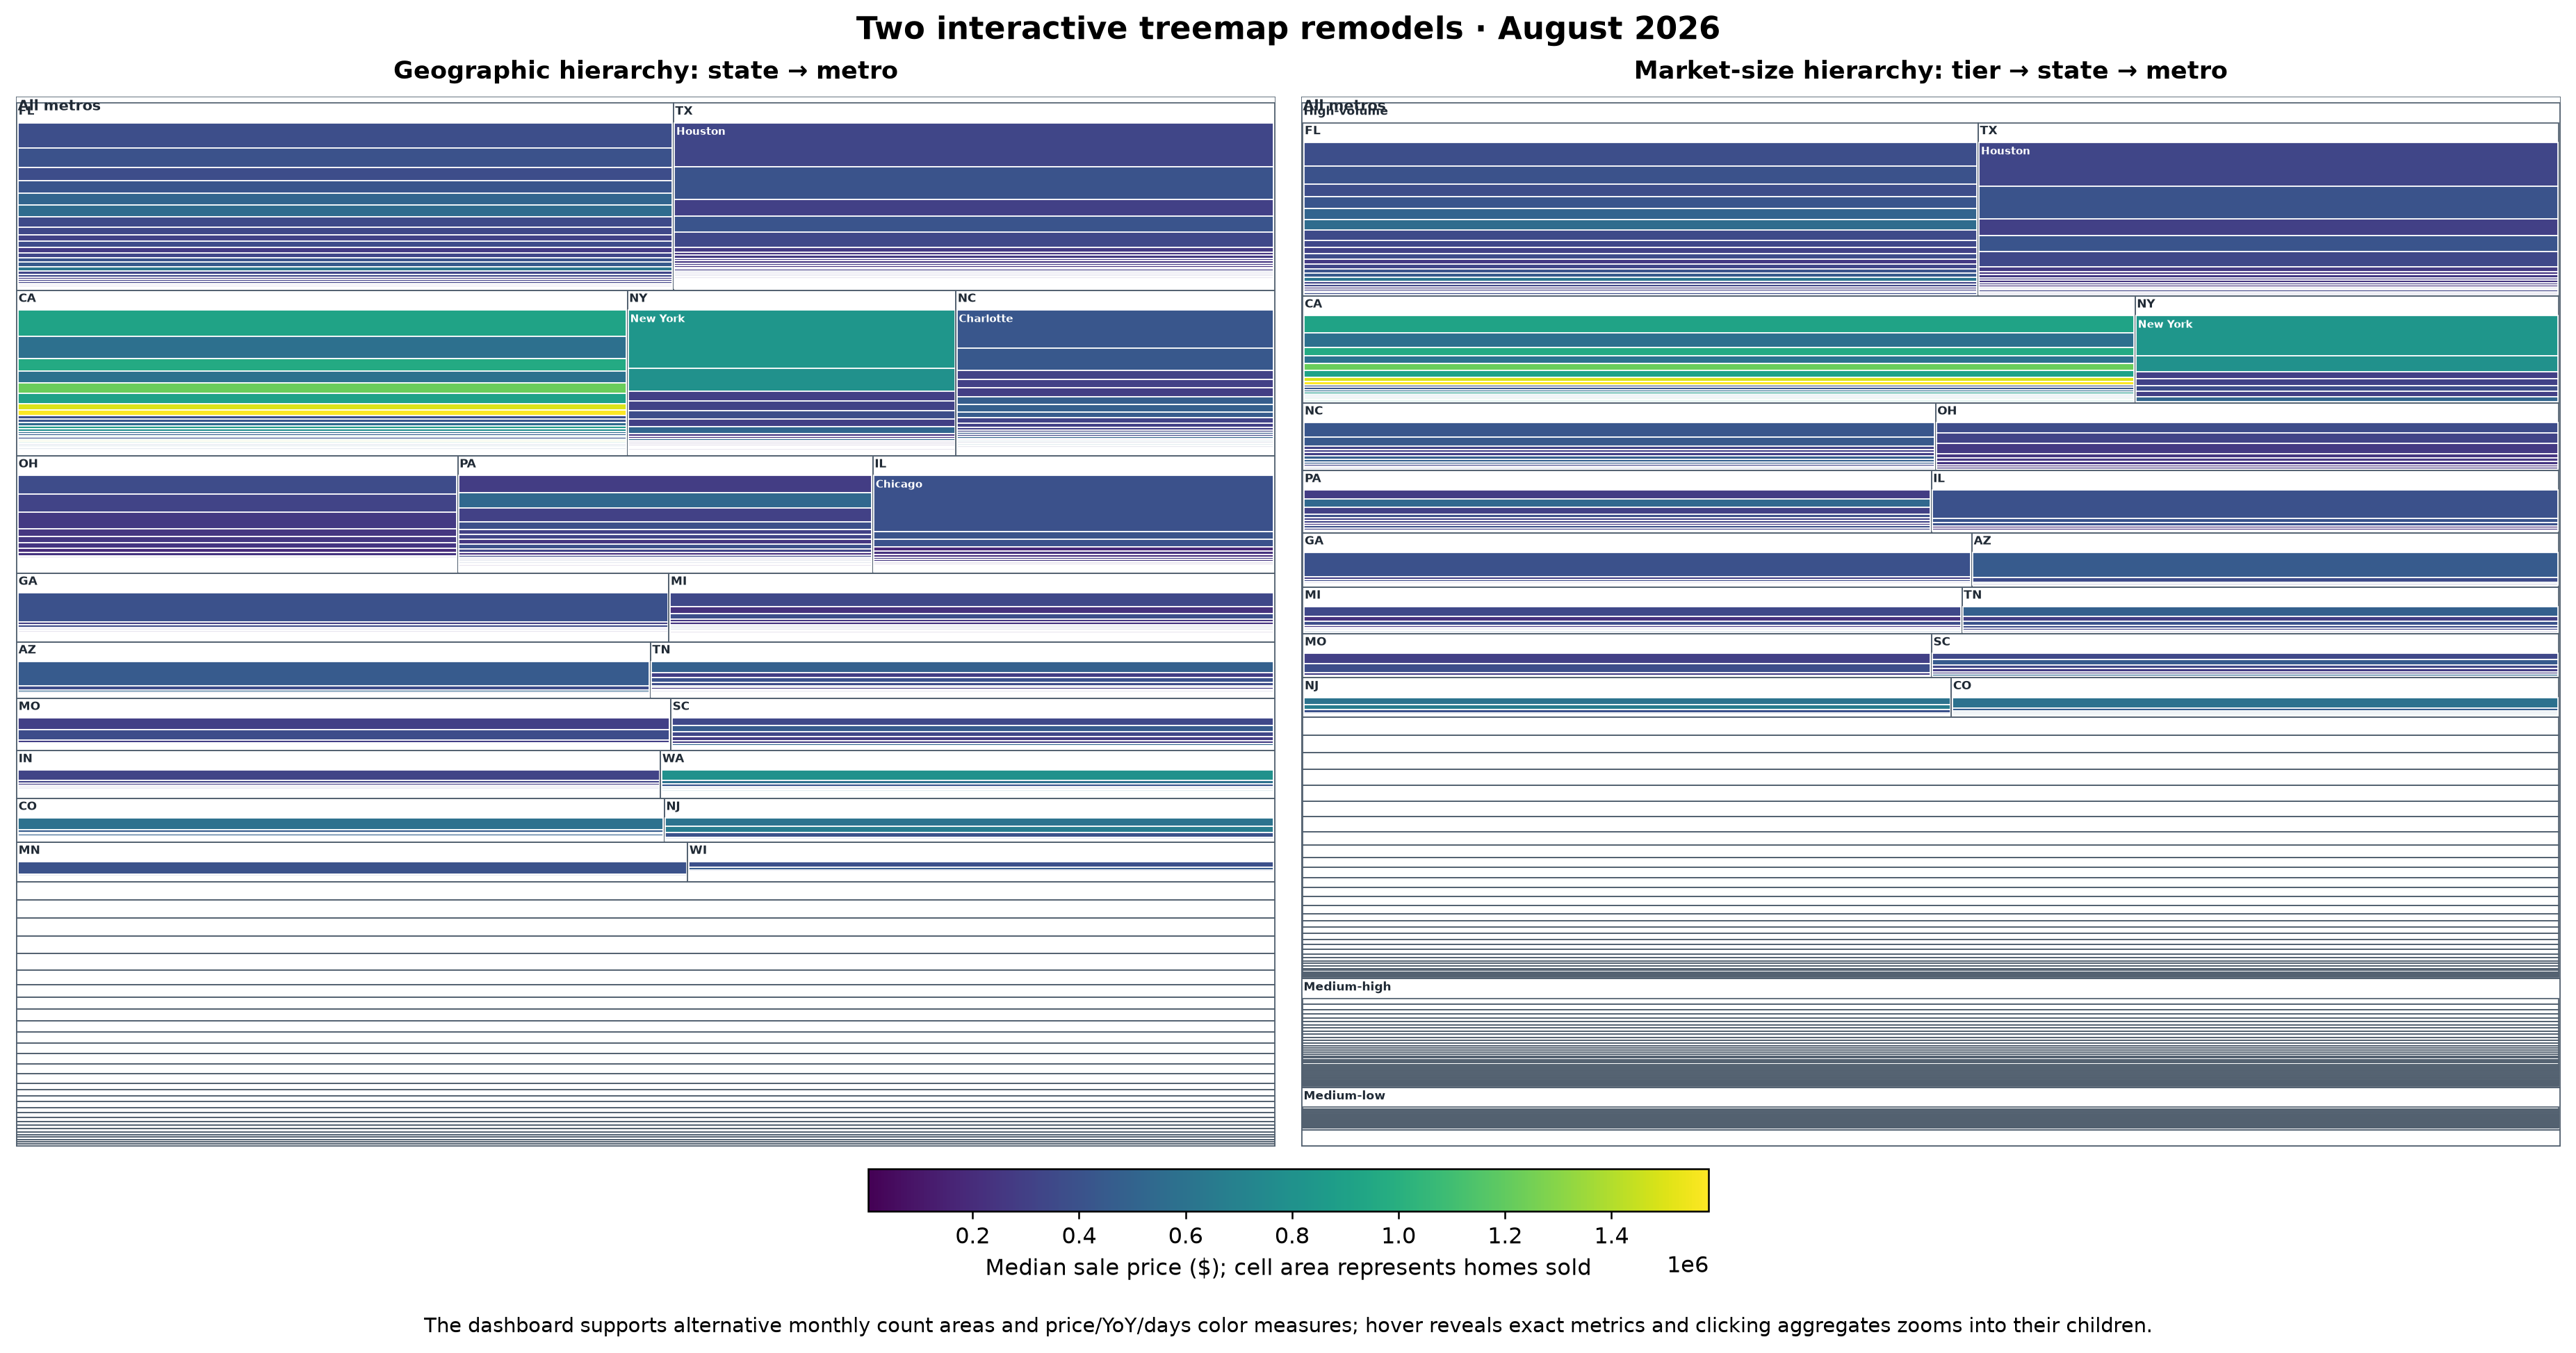
\includegraphics[width=\textwidth]{fig_treemap_hierarchy_comparison.png}
\caption{Alternative treemap remodels: state--metro and market-size tier--state--metro. Rectangle area represents an additive monthly market measure; color represents a selected indicator. The live view adds month and measure selectors, zoom, breadcrumbs, and detailed hover values.}
\label{fig:treemap}
\end{figure}

Figure~\ref{fig:treemap} illustrates the trade-off between the two hierarchies. State--metro is easier to interpret geographically, while tier--state--metro makes the relative contribution of market-size classes visible before drilling into state and metro. Area should be used for comparing large totals, not for precise comparison of similarly sized small rectangles. Color adds a second measure but is affected by the robust display range; exact tooltip values are necessary for precise reading.

\subsection{Horizon and ridgeline plots}\label{sec:temporal}
The time-series figures are generated with Python scientific plotting libraries (pandas for aggregation and Matplotlib for plotting). Horizon plots share a zero baseline and use layered bands to compress variation into small multiples. The price-change view folds values in 5-percentage-point bands and groups metros by fixed market-size tier. The DOM-change view folds values in 10-day bands and groups metros by Census region. In both cases, positive values appear above zero and negative values below zero; the band stack encodes magnitude. Group medians are plotted for each month to limit sensitivity to extreme metro observations.

\begin{figure}[H]
\centering
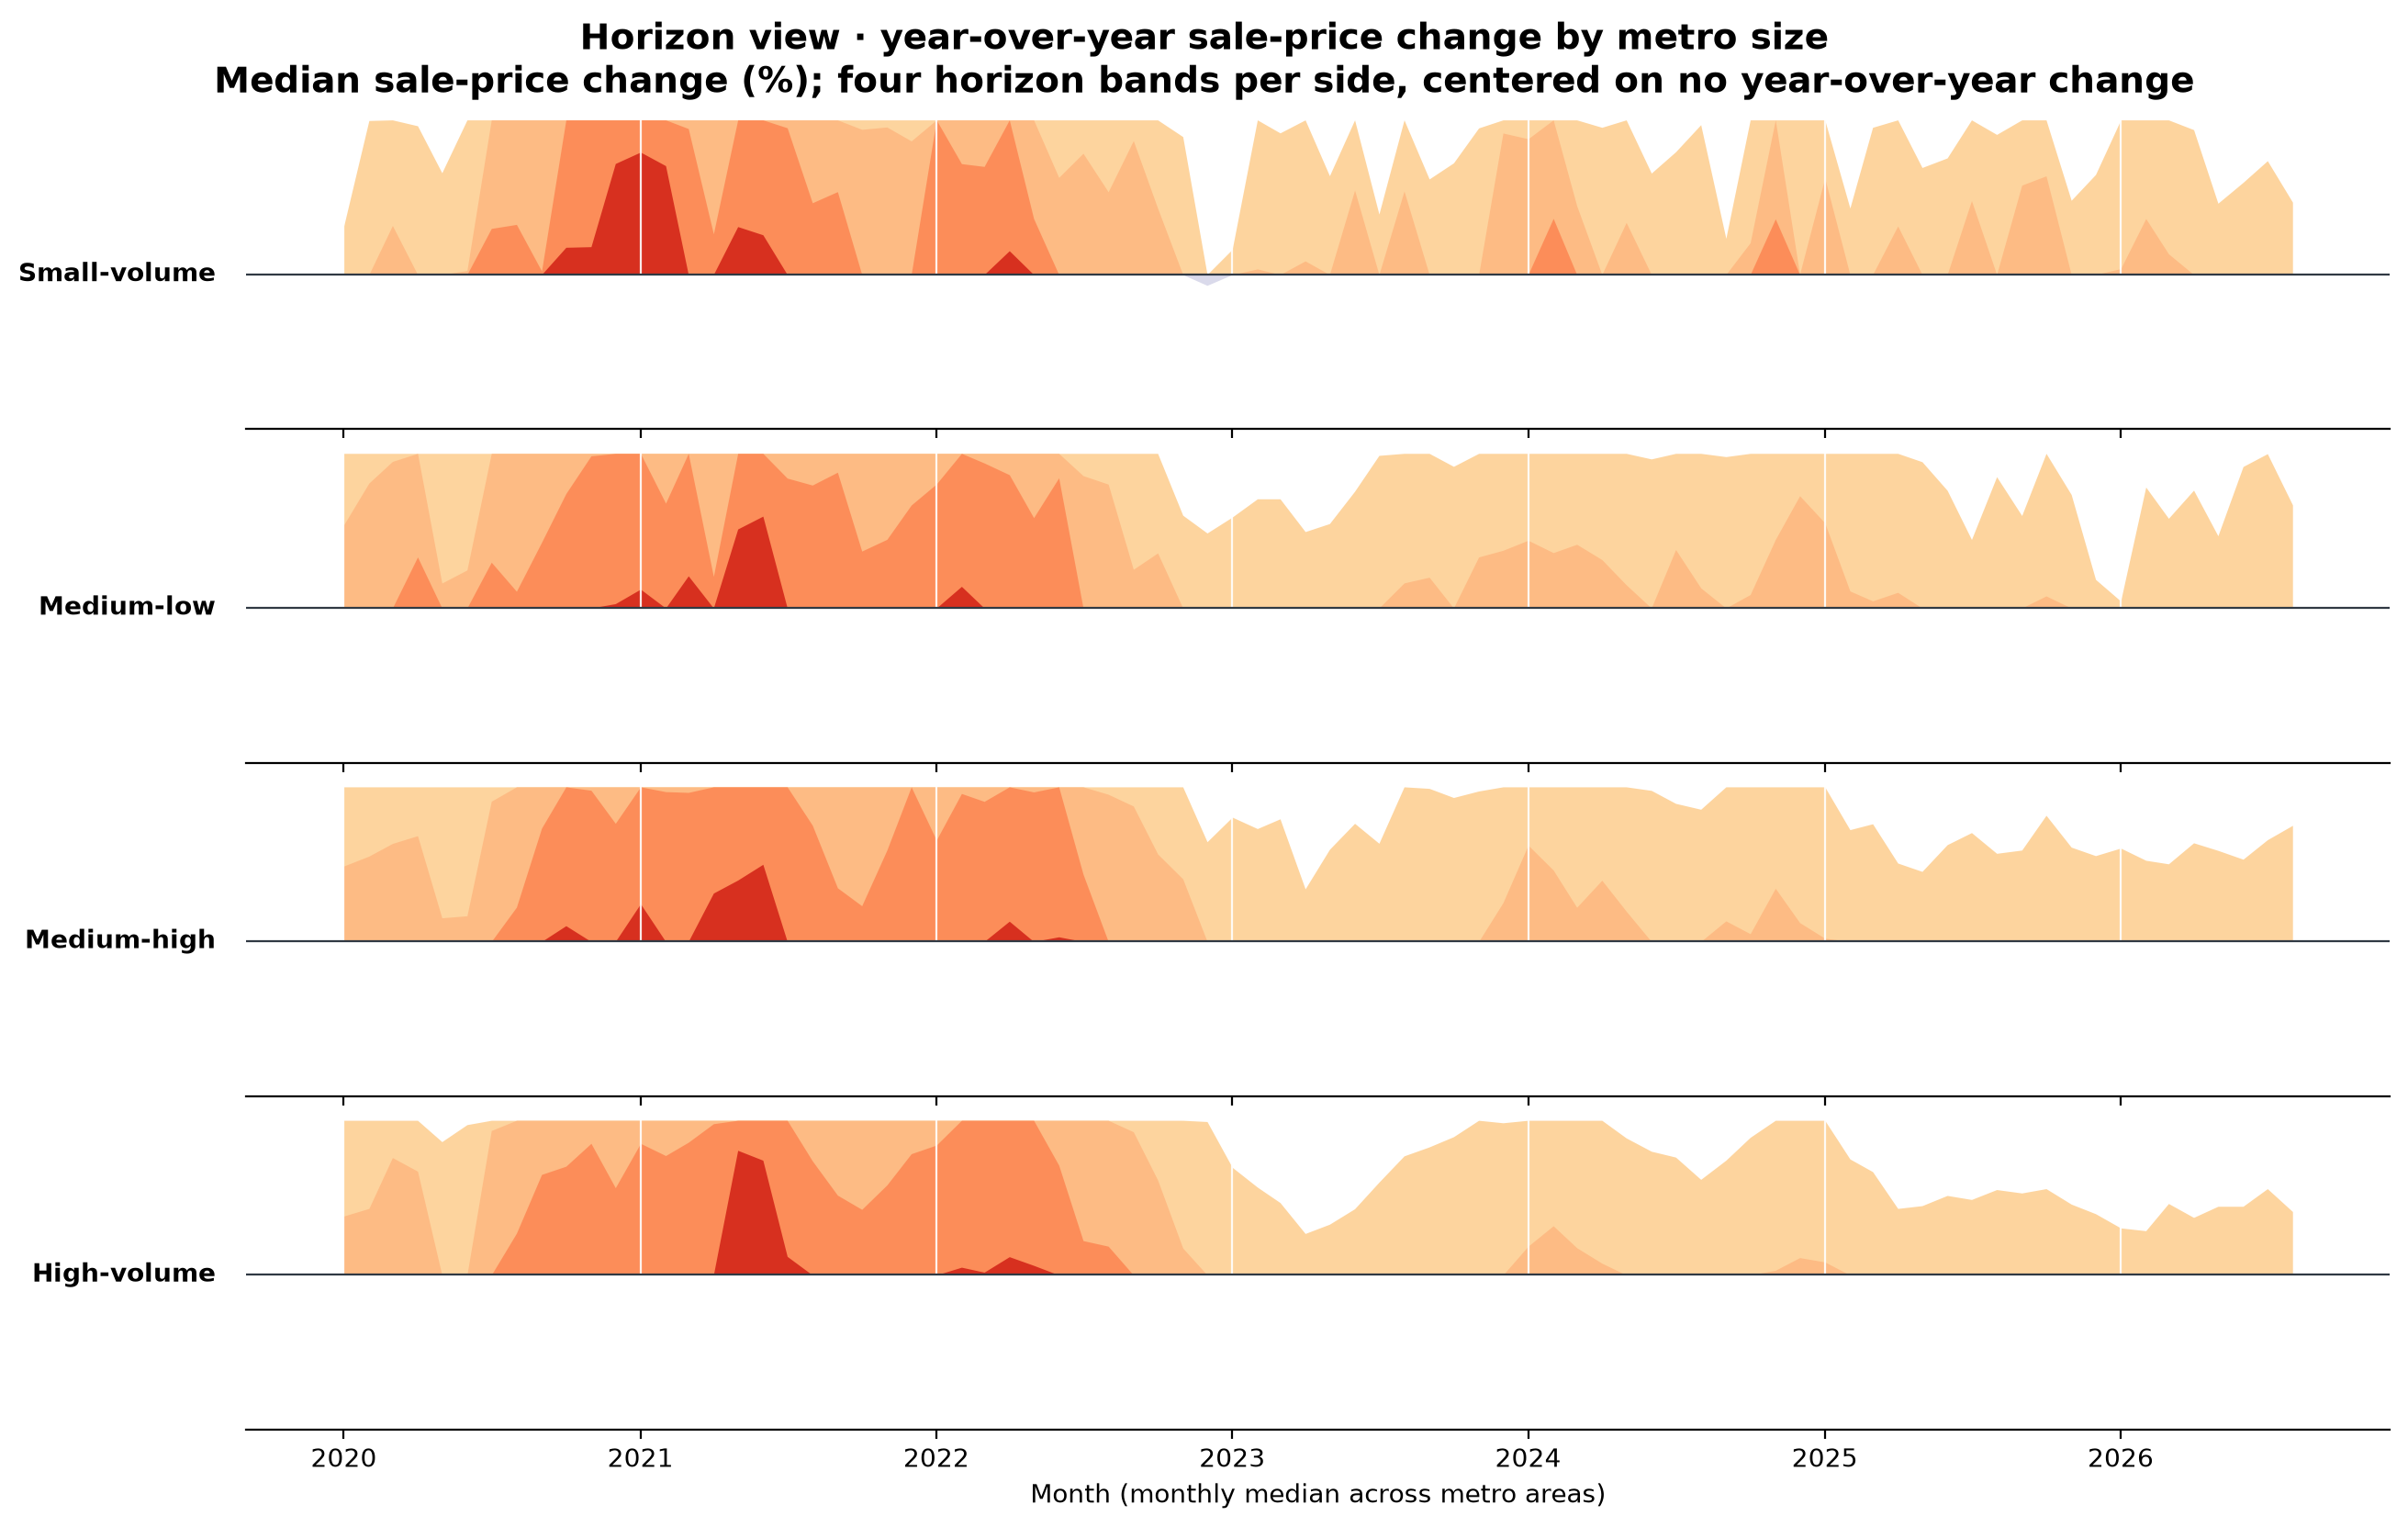
\includegraphics[width=0.98\textwidth]{redfin_horizon_price_yoy.png}
\caption{Horizon variation 1: monthly median year-over-year sale-price change by fixed metro-size tier, January 2020--August 2026. Each band represents five percentage points around zero.}
\label{fig:horizon-price}
\end{figure}

\begin{figure}[H]
\centering
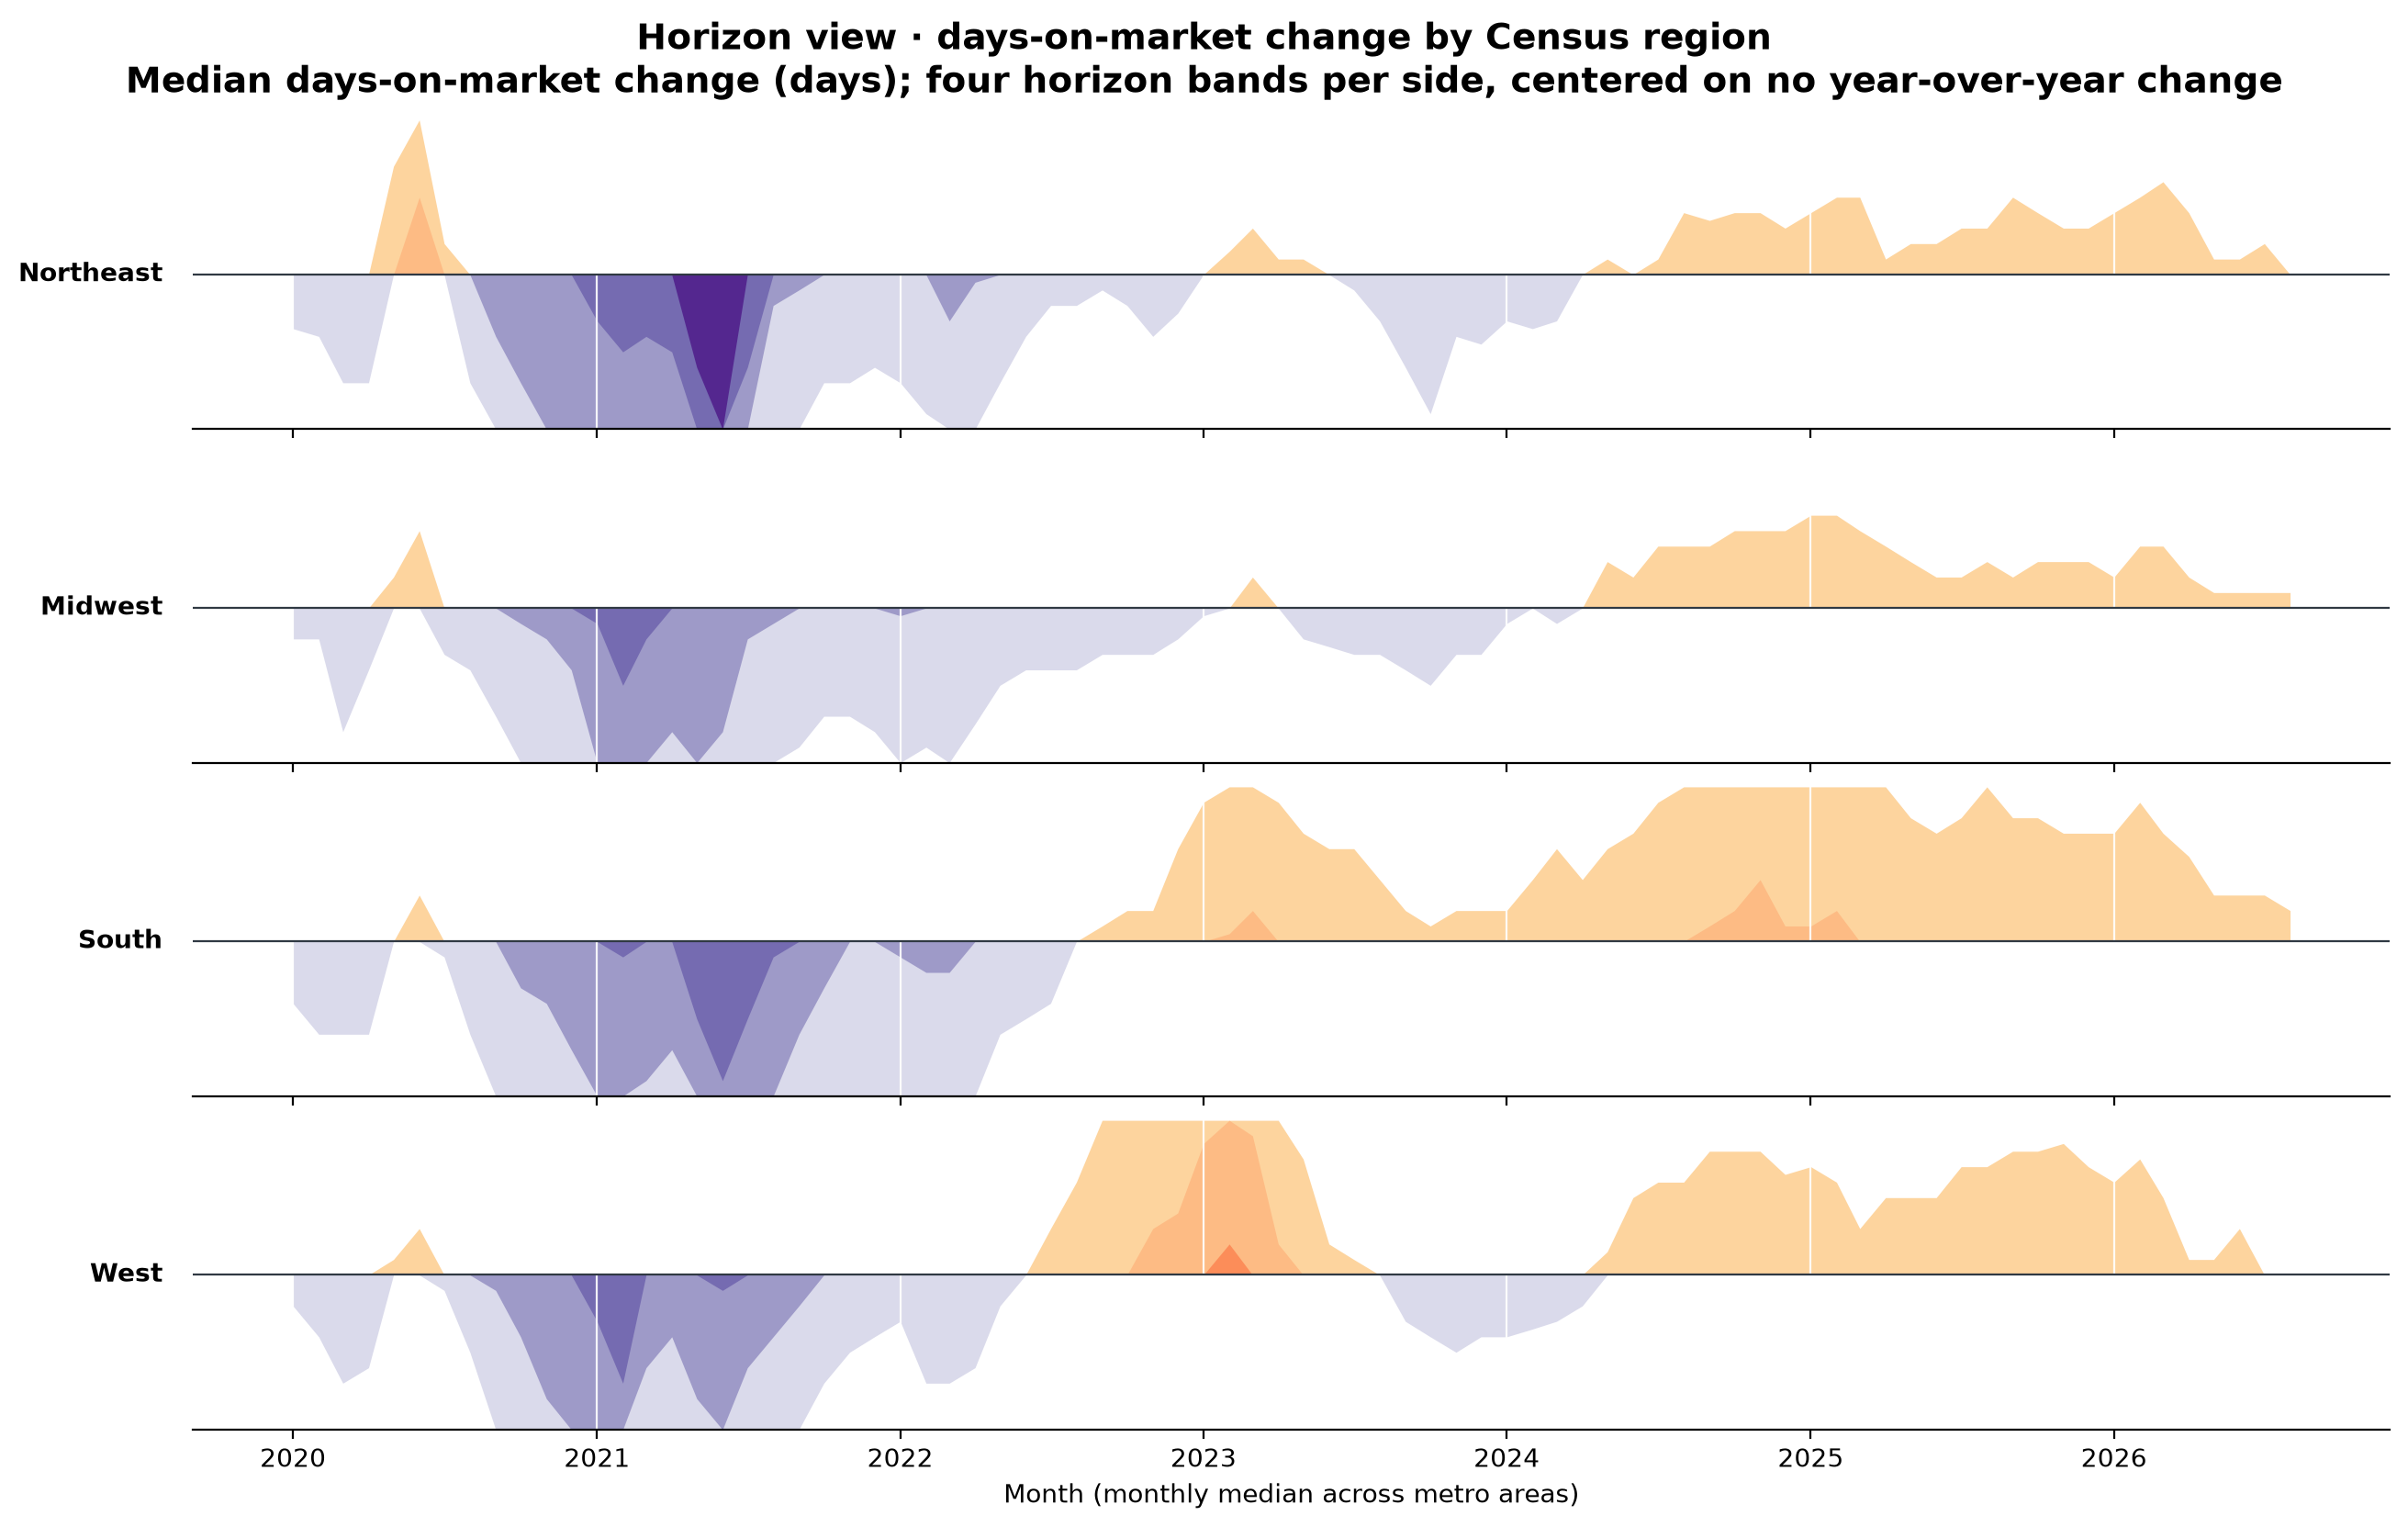
\includegraphics[width=0.98\textwidth]{redfin_horizon_days_yoy.png}
\caption{Horizon variation 2: monthly median year-over-year DOM change by Census region, January 2020--August 2026. Each band represents ten days; positive values mean homes took longer to sell than one year earlier.}
\label{fig:horizon-dom}
\end{figure}

The price horizon (Figure~\ref{fig:horizon-price}) shows the strong price-growth period around 2020--2022 followed by slower positive year-over-year growth across groups. Group differences are visible: in recent years the smaller-volume tiers generally retain somewhat higher price-growth medians than the high-volume tier. A positive median indicates that the typical metro in that group had a higher sale-price indicator than one year before; it does not mean every metro rose. The DOM horizon (Figure~\ref{fig:horizon-dom}) records a sharp period of faster selling relative to the previous year around 2021, followed by a shift toward positive DOM changes in later years. This is consistent with a cooling in selling speed at the group-median level. Regional differences exist, but all regions share broad temporal phases.

For ridgelines, each curve is a smoothed density estimate over a group distribution. The annual-price view contains one annual median sale price per metro, grouped by year; a logarithmic horizontal scale keeps lower- and higher-priced metros visible together. The DOM view uses each metro's median DOM over the latest 12 months and groups it by the four fixed metro-size tiers. Its horizontal display is clipped at the 99th percentile to avoid a few extreme values dominating the shape; the sample count and scale are shown in the plot.

\begin{figure}[H]
\centering
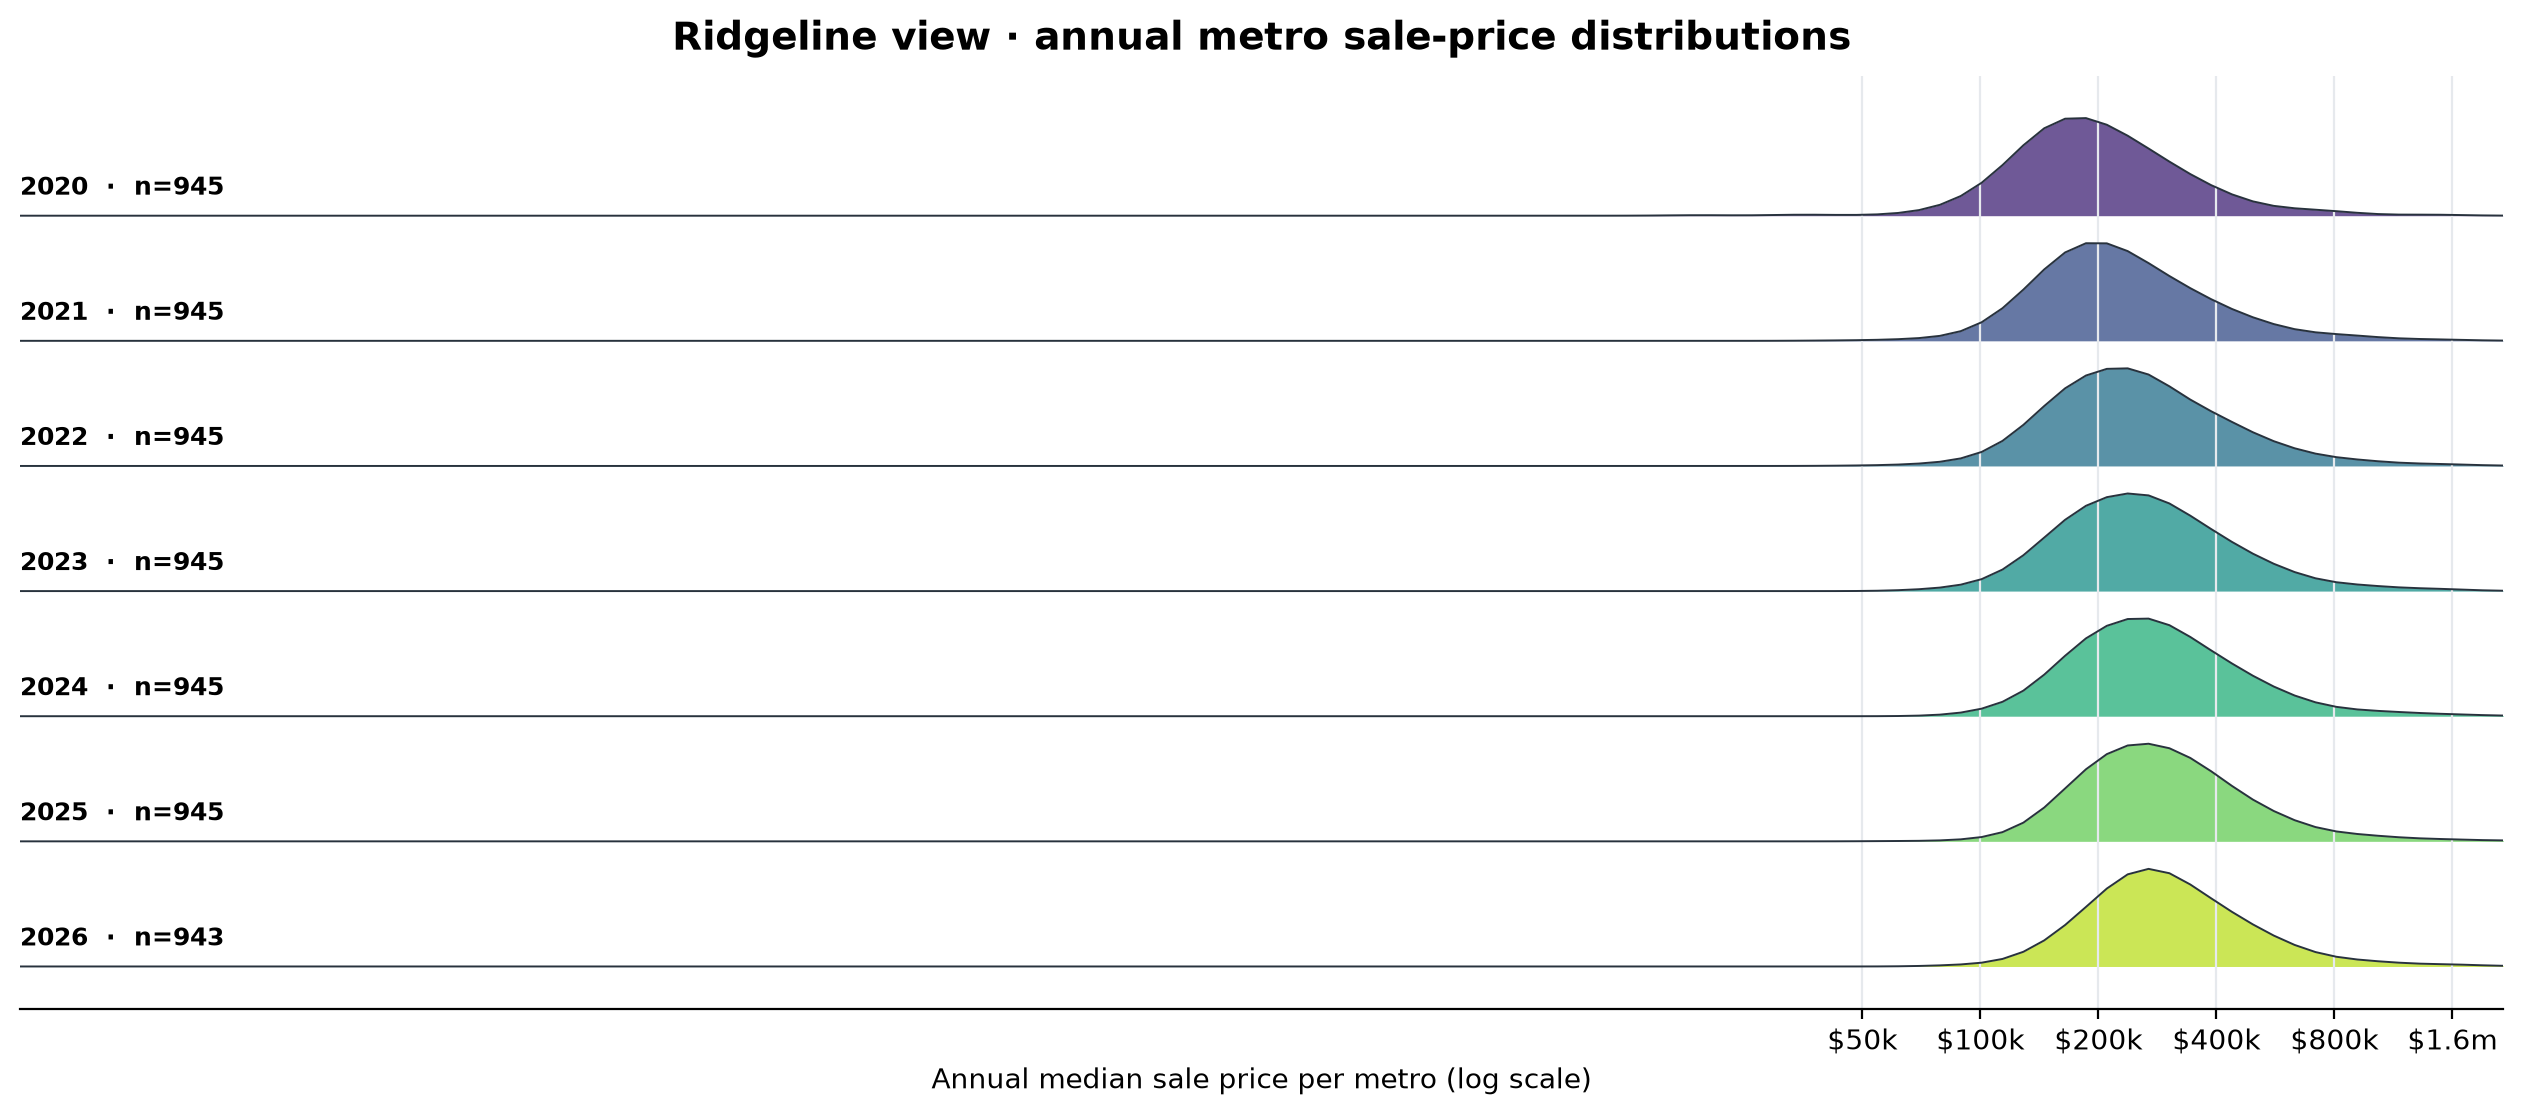
\includegraphics[width=0.98\textwidth]{redfin_ridgeline_price_by_year.png}
\caption{Ridgeline variation 1: distributions of metro-level annual median sale prices for 2020--2026. The 2026 distribution covers January--August only; the horizontal axis is logarithmic.}
\label{fig:ridge-price}
\end{figure}

\begin{figure}[H]
\centering
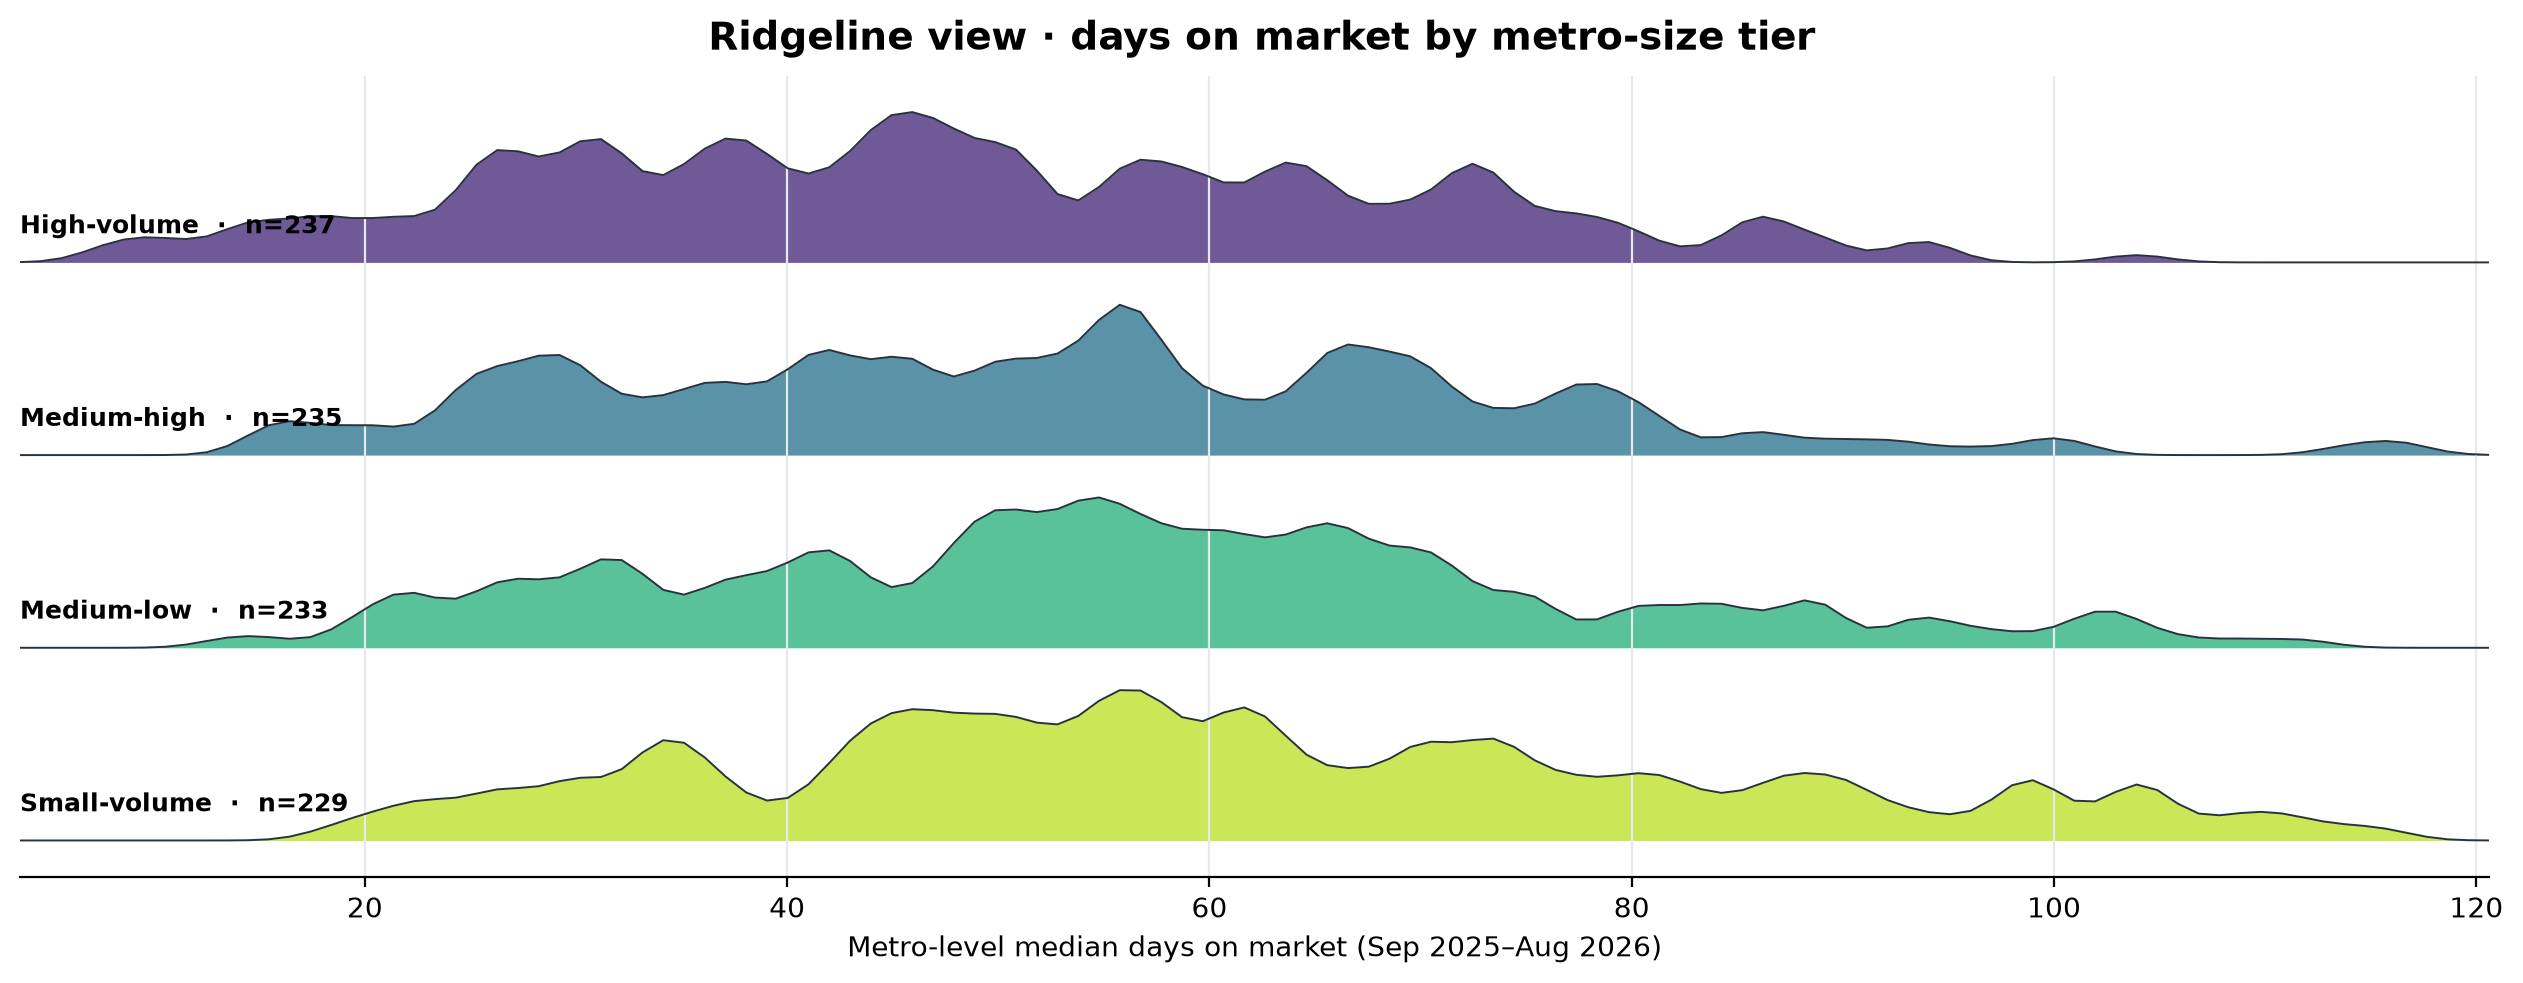
\includegraphics[width=0.98\textwidth]{redfin_ridgeline_days_by_tier.png}
\caption{Ridgeline variation 2: distributions of metro-level median DOM over September 2025--August 2026, grouped by fixed market-size tier. The display is clipped at the 99th percentile.}
\label{fig:ridge-dom}
\end{figure}

The annual-price ridgeline (Figure~\ref{fig:ridge-price}) shifts to the right across years, indicating a broad increase in metro-level price distributions. The 2026 curve is partial and should not be treated as a full-year result. The latest-year DOM ridgeline (Figure~\ref{fig:ridge-dom}) shows different distribution centers and spreads across market-size tiers. In the data, the median of metro-level 12-month DOM summaries is about 47.5 days in high-volume metros and about 60.5 days in small-volume metros, with the two middle tiers between these values. This describes a group-level association in this dataset and period; it does not establish that metro size causes a faster sale.

\section{Cross-view findings}
Across the Redfin views, the main pattern is a broad increase in sale prices over the study period alongside a deceleration in year-over-year price growth after the rapid gains of 2020--2022. The monthly median sale-price change falls from double-digit levels in 2021 to low single digits in the most recent years. At the same time, DOM changes turn positive after the especially fast-selling conditions around 2021, suggesting that sales generally took longer than a year earlier in later periods. The fixed-tier and region views show that this broad pattern is not perfectly uniform: the magnitude and timing vary among groups.

The treemap and parallel coordinates serve different purposes. The treemap emphasizes composition and additive scale for a selected month, while the parallel plot emphasizes multivariate profiles and conditional comparisons across metros. Treemap colors should not be read as area totals; parallel-coordinate bundles should not be read as unmodified individual trajectories. Together with hover values and filtering, these views help validate broad patterns and examine exceptions.

The network findings describe a different phenomenon. The highly active pages and strong transitions reveal concentrated activity in the selected clickstream core. Since the core preserves less than one percent of internal-link clicks and excludes the long tail by design, its apparent hubs and communities should be interpreted as properties of a high-activity induced subgraph, not a census of all Wikipedia navigation.

\section{Interaction and software design}
The dashboard groups each task into a dedicated tab, with controls next to the relevant visualization. Interaction follows a consistent inspect-and-filter pattern: choose a layout or grouping, apply a filter, inspect a mark using hover details, and reset or navigate back when needed. The browser views use JavaScript and D3 for graph and housing interactions; NetworkX and Python perform network construction and layout calculations; pandas and Matplotlib prepare and render the temporal small multiples. This division preserves responsive in-browser exploration while keeping data preparation and statistical aggregation explicit.

The images in this report are static evidence of the main encodings. The live dashboard provides the interaction states that cannot be represented in a single image. The application README and source files document the environment and entry point; the main implementation files are \texttt{app.js}, \texttt{prepare\_infovis.py}, and \texttt{prepare\_redfin.py}, with styles in \texttt{styles.css}. The report figures are stored in \texttt{images/}.

\section{Limitations and interpretation safeguards}
\begin{enumerate}[leftmargin=*]
  \item \textbf{Network selection.} Selecting the 120 most active pages creates a readable core but excludes most pages and approximately 99.39\% of internal-link click volume. Network centrality, communities, and layout patterns are conditional on that selection.
  \item \textbf{Aggregated counts.} Clickstream counts are aggregate transitions. They do not identify individuals, sessions, intent, or chronology. No temporal claim is made about the network.
  \item \textbf{Layout variability.} Force-directed layouts may depend on initialization and algorithm parameters. The implementation fixes seeds where supported for repeatability, but the coordinates themselves are not semantic measurements.
  \item \textbf{Missing data.} The Redfin data contain missing metro-month observations and missing indicator fields. The parallel view omits incomplete records for displayed axes; group summaries are calculated from available values. Small differences in group coverage can affect comparisons.
  \item \textbf{Partial 2026.} The source ends in August 2026. Annual 2026 prices are based on eight months and must not be compared as a complete year without this qualification.
  \item \textbf{Aggregation.} Medians summarize groups and mask within-group variation. Treemap parent colors are area-weighted means of metro-level indicators, not necessarily official aggregate statistics. Ridgeline smoothing can hide local modes, and the DOM figure clips the far tail for display.
  \item \textbf{No causal identification.} Regional and metro-size contrasts are descriptive. They do not establish why market values or selling times changed.
\end{enumerate}

\section{Conclusion}
The InfoVis implementation addresses the three task families with complementary views: a NetworkX click-flow core compared under three layouts, an interactive Redfin parallel-coordinates plot with edge bundling, two zoomable treemap hierarchies, and two variations each of horizon and ridgeline plots. The combination is useful because each view answers a different question: connectivity and layout for click flows, multivariate profiles for metro comparisons, hierarchical composition for monthly totals, and distributions or temporal change for market trends.

The data support a descriptive account of rising metro price distributions, slower price appreciation after 2022, and a shift toward longer selling times relative to the prior year after the fast-selling period around 2021. The group comparisons show meaningful variation by metro size and region. These conclusions are limited by aggregation, missing observations, partial 2026 coverage, and the intentionally restricted clickstream core. The report and dashboard therefore pair summary patterns with filters and exact-value tooltips to support closer inspection.

\section{Team contributions}\label{sec:contrib}
Replace the placeholders with the actual team roster. Edit or remove rows so every member has a distinct task owner; data cleaning may be listed separately, but the assignment does not permit joint ownership of visualization tasks.

\begin{table}[H]
\centering
\begin{tabularx}{\textwidth}{p{0.27\textwidth}Y}
\toprule
\textbf{Team member} & \textbf{Individual contribution (edit to match actual work)} \\
\midrule
\memberA & [Network data preparation, NetworkX graph, layout comparison and interaction implementation.] \\
\memberB & [Redfin parallel coordinates, edge bundling, brushing and axis-reordering implementation.] \\
\memberC & [Treemap hierarchy experiments, temporal plots, analysis and report integration.] \\
\bottomrule
\end{tabularx}
\caption{Editable contribution record. Ensure the final division reflects the work actually completed and has no duplicated visualization ownership.}
\label{tab:contrib}
\end{table}

\section*{Artifact checklist}
\addcontentsline{toc}{section}{Artifact checklist}
\begin{itemize}[leftmargin=*]
  \item Report source: \texttt{infovis\_report.tex}.
  \item Network comparison image: \texttt{images/fig\_network\_layout\_comparison.png}.
  \item Parallel-coordinate and treemap comparison images: \texttt{images/fig\_parallel\_coordinates\_bundling.png} and \texttt{images/fig\_treemap\_hierarchy\_comparison.png}.
  \item Four Python-generated temporal figures: the two \texttt{redfin\_horizon\_*} images and two \texttt{redfin\_ridgeline\_*} images in \texttt{images/}.
  \item Interactive application and preparation code: \texttt{index.html}, \texttt{app.js}, \texttt{prepare\_infovis.py}, and \texttt{prepare\_redfin.py}.
\end{itemize}

\begin{thebibliography}{9}
\bibitem{assignment} DAS732: Data Visualization, Term 1 (2026--27), \emph{Programming Assignment 2: Familiarization with SciVis and InfoVis Methods}, assignment brief supplied with the course.
\bibitem{clickstream} Wikimedia Foundation, \emph{Wikipedia Clickstream}, dataset and documentation, \url{https://meta.wikimedia.org/wiki/Research:Wikipedia_clickstream}.
\bibitem{redfin} Redfin, \emph{Data Center: Download Housing Market Data}, \url{https://www.redfin.com/news/data-center/downloads/}.
\bibitem{networkx} NetworkX Developers, \emph{Drawing and Layout}, NetworkX documentation, \url{https://networkx.org/documentation/stable/reference/drawing.html}.
\bibitem{d3treemap} D3.js, \emph{Treemap}, D3 Hierarchy documentation, \url{https://d3js.org/d3-hierarchy/treemap}.
\bibitem{d3brush} D3.js, \emph{Brush}, D3 documentation, \url{https://d3js.org/d3-brush}.
\end{thebibliography}

\end{document}
